\documentclass[psamsfonts]{amsart}

% -------Packages---------
\usepackage{microtype}[final]
\usepackage[style=numeric]{biblatex}
\usepackage{hyperref}
\addbibresource{/home/philip/documents/text/references/bibliography.bib}
\usepackage{amssymb,amsfonts}
\usepackage[all,arc]{xy}
\usepackage{enumerate}
\usepackage{mathrsfs}
\usepackage{todonotes}
\usepackage{tikz}
\usetikzlibrary{automata,positioning,shapes}
\usepackage[nolist]{acronym}

%--------Theorem Environments--------
%theoremstyle{plain} --- default
\newtheorem{thm}{Theorem}[section]
\newtheorem{cor}[thm]{Corollary}
\newtheorem{prop}[thm]{Proposition}
\newtheorem{lem}[thm]{Lemma}
\newtheorem{conj}[thm]{Conjecture}
\newtheorem{quest}[thm]{Question}
\newtheorem{prob}[thm]{Problem}

\theoremstyle{definition}
\newtheorem{defn}[thm]{Definition}
\newtheorem{defns}[thm]{Definitions}
\newtheorem{con}[thm]{Construction}
\newtheorem{exmp}[thm]{Example}
\newtheorem{exmps}[thm]{Examples}
\newtheorem{notn}[thm]{Notation}
\newtheorem{notns}[thm]{Notations}
\newtheorem{addm}[thm]{Addendum}
\newtheorem{exer}[thm]{Exercise}
\newtheorem{fact}[thm]{Fact}

\theoremstyle{remark}
\newtheorem{rem}[thm]{Remark}
\newtheorem{rems}[thm]{Remarks}
\newtheorem{warn}[thm]{Warning}
\newtheorem{sch}[thm]{Scholium}


\makeatletter
\let\c@equation\c@thm
\makeatother
\numberwithin{equation}{section}

\title{Undecidability and the structure of the Turing degrees}

\author{Philip Adams}

\date{\today}

\begin{document}

\begin{abstract}

  This paper explores the structure and properties of the Turing degrees, or
  degrees of undecidability. We introduce the Turing machine, an abstract model
  of computation, in order to develop the concepts of undecidability and Turing
  reduction. We demonstrate the technique of proof by reduction through a series
  of examples of undecidable problems related to context-free grammars. We then
  employ reducibility to consider a partial ordering on the set of Turing degrees, $\mathcal{D}$. Finally, we prove a variety of theorems
  related to the structure of $\mathcal{D}$.
  
\end{abstract}

\maketitle


\tableofcontents
\begin{acronym}
  \acro{PDA}[PDA]{Pushdown Automaton}
  \acroplural{PDA}[PDAs]{Pushdown Automata}
  \acro{DPDA}[DPDA]{Deterministic Pushdown Automaton}
  \acroplural{DPDA}[DPDAs]{Deterministic Pushdown Automata}
  \acro{TM}[TM]{Turing Machine}
  \acro{FSA}[FSA]{Finite State Automaton}
  \acroplural{FSA}[FSAs]{Finite State Automata}
  \acro{CFG}[CFG]{Context-Free Grammar}
  \acro{CFL}[CFL]{Context-Free Language}
  \acro{DCFL}[DCFL]{Deterministic Context-Free Language}
\end{acronym}

\section{Introduction}
Historical overview of the field, motivation for study
\cite{ambos-spies06:_degrees_unsol}
\cite{soare16_turin_comput}
\cite{soare1999history}
\cite{lerman16:_degrees_unsol}
\todo{}
\subsection{Decision Problems}
What does it mean to \emph{solve a problem}? What is a \emph{problem}, anyways?
These questions may seem superfluous, they must be addressed in order to build a
well defined theory of the difficulty of problems. In this paper, we discuss a
specific type of problem, the \emph{decision problem}. Decision problems are
essentially sets of natural numbers, and to solve the problem is to be able to
decide whether any given element is inside the set or not. Because set theory is
commonly used as the foundational system of mathematics, we can convert problems
expressed in terms of more complex mathematical objects into decision problems,
and thus by studying decision problems can build a system that is able to assess
the computability of all mathematical problems. For example, we can express
strings over the alphabet $\{0,1\}$ as sets of natural numbers, and thus can
study problems about languages of such strings with the same tools we use for
decision problems. Going further, we can express the source code of a computer
program as a string over the alphabet $\{0,1\}$, and so can consider questions
about the behavior of computer programs.


\section{Models of Computation}
Upon consideration of different types of problems, it quickly becomes clear that
some are much more difficult than others. For example, when considering words
over the alphabet $\{a,b,c\}$, it seems much easier to determine whether a word
ends in an $a$ than whether a word is a palindrome. It seems even harder still
to determine whether the word is of the form $a^nb^nc^n$. In order to formalize
these notions of difficulty, we need to build abstract models of computation,
and then test their ability to decide such questions. We observe that a machine
that can solve the first problem only needs to ``remember'' the same amount of
information no matter how long the input is: the last letter of the word. In
contrast, the amount of memory that the second and third problems require is
dependent on the size of the input, because the first half of the palindrome or
$n$, respectively, can be arbitrarily large. The difference between the second
and third problems is more subtle: the second problem can be solved moving only
one direction in memory, while the third problem requires the ability to ``look
back'' in memory.
\par
Based on these differences, we can begin to construct different models of
computation that have just enough power to solve each problem. The first problem
can be solved by a \emph{\ac{FSA}}, a collection of a finite
number of states, a transition function, and a set of accepting states. The
\ac{FSA} accepts the input if the sequential application of each element to the
input finishes in an accepting state, and rejects otherwise. \aclp{FSA} are often represented by charts as in Figure~\ref{fig:fsa}, a
representation of an \ac{FSA} that decides the first problem.
\begin{figure}[h]
  \caption{An \ac{FSA} that determines whether a string ends in
    `$a$'.}
  \label{fig:fsa}
  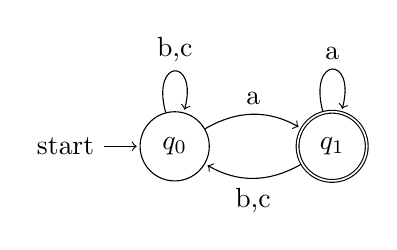
\begin{tikzpicture}[shorten >=1pt,node distance=2cm,on grid,auto]
  \node[state,initial] (q_0) {$q_0$};
  \node[state,accepting] (q_1) [right=of q_0]{$q_1$};
  \path[->]
  (q_0) edge [loop above] node {b,c} ()
  edge [bend left] node  {a} (q_1)
  (q_1) edge [bend left] node {b,c} (q_0)
  edge [loop above] node {a} ();
\end{tikzpicture}
\end{figure}
\par
The second problem can be solved by a machine called a \emph{\ac{PDA}}, which is essentially a finite state automaton with the addition of
a stack. Rather than transforming the current state and the input into a new
state, as with a finite state automata, the transition function of a \ac{PDA} also considers the stack, which it can pop and push from. Within the
collection of \acp{PDA}, there is another division between
\emph{\acp{DPDA}} and \emph{Nondeterministic \aclp{PDA}}. For \acp{DPDA}, the
transition function only outputs one move, rather than a set of
moves. Nondeterministic \acp{PDA} are able to recognize more languages than
\acp{DPDA}. Figure~\ref{fig:pda} is a graphical representation of a \ac{PDA}
that decides palindromes. In this representation, $\epsilon$ is an empty input,
and  is a special symbol that denotes the bottom of the stack. The moves are
represented by a double of input and stack operation.

\begin{figure}[h]
  \label{fig:pda}
  \caption{A \acl{PDA} that decides palindromes over the alphabet ${a,b}$}
  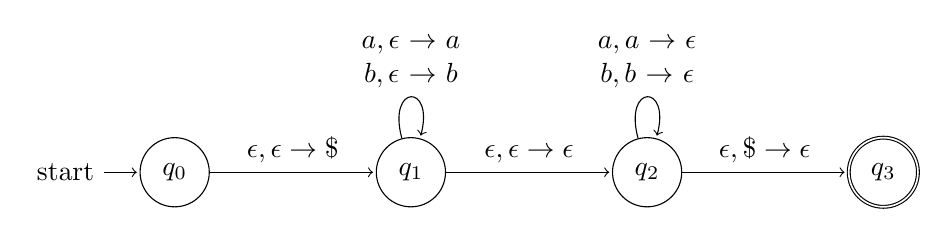
\begin{tikzpicture}[shorten >=1pt,node distance=3cm,on grid,auto]
  \node[state,initial] (q_0) {$q_0$};
  \node[state] (q_1) [right=of q_0]{$q_1$};
  \node[state] (q_2) [right=of q_1]{$q_2$};
  \node[state,accepting] (q_3) [right=of q_2]{$q_3$};
  \path[->]
  (q_0) edge node {$\epsilon,\epsilon\to\$$} (q_1)
  (q_1) edge [loop above] node[text width=1.5cm,align=center] {$a,\epsilon\to a$
    $b,\epsilon\to b$} ()
  edge node {$\epsilon,\epsilon\to\epsilon$} (q_2)
  (q_2) edge [loop above] node[text width=1.5cm,align=center] {$a,a\to\epsilon$
    $b,b\to\epsilon$} ()
  edge node {$\epsilon,\$\to\epsilon$} (q_3);  
  \end{tikzpicture}
\end{figure}

\subsection{Turing Machines}
Finally, we arrive at the \ac{TM}, devised by Alan Turing in his paper \emph{On
  Computable Numbers, With an Application To the Entscheidungsproblem}
~\cite{turing37_comput_number_with_applic_to_entsc}. \aclp{TM} offer an
unrestricted model of computation, equivalent to the general purpose computers
that we are familiar with today. This equivalence is expressed by a pair of
concepts called \emph{Turing completeness} and \emph{Turing equivalence}. A
system of computation is Turing complete if it is able to simulate an arbitrary
Turing machine, and is Turing Equivalent if there is a Turing machine that can
simulate it. Essentially, Turing completeness is being \emph{at least} as
powerful as Turing machines, while Turing equivalence is being \emph{exactly} as
powerful as a Turing machine. Turing machines are themselves Turing complete, as are other
abstract models of computation such as the \emph{lambda calculus}. General
purpose programming languages are also considered Turing complete, because
although they are run on real machines with finite storage space, this space is
theoretically unbounded, and thus the expressive power of the languages are
unbounded even if any particular instance of a program run on an actual machine
would not be able to simulate all Turing machines. 
\par
A basic informal definition of a Turing machine is a collection of an infinite tape
of discrete cells,
a head that can move back and forth between cells on the tape as well as read and write
from the tape, a register that stores the current state of the machine out of a
finite set of possible states and starts in a start state, a set of accepting
states, and a transition function that at each step allows tells the machine
wether to write to the tape, move the head, or change states. There are
modifications to this definition which allow for multiple tapes or
nondeterminism, but they are all equivalent to the basic
definition. Additionally, a \ac{PDA} with two stacks is equivalent to a Turing
machine, as the stacks can be thought of as extending out in opposite
directions, forming an infinite tape.

\section{Undecidability}
In the previous section we were concerned primarily with problems that our
models of computation were able to solve. However, much as an \ac{FSA} is unable
to solve the problem of whether a string is a palindrome, there are problems
that are too difficult for even \aclp{TM} to solve. When a decision problem $A$
cannot be solved by a model $\mathcal{M}$, we say that $A$ is undecidable for
$\mathcal{M}$. When we just say that $A$ is undecidable, we mean that it is
undecidable for \acp{TM}. \par
It can be difficult to come up with obvious examples of problems that are
undecidable. After all, we usually talk about sets based on the patterns they
exhibit, and those patterns are typically simple enough to be enumerated by a
computer. A promising place to look for problems that a model cannot decide is
problems about the model itself, and the most famous undecidable problem is of
that type. The Halting Problem, introduced by Alan Turing in the same paper
where he introduced the Turing machine, asks whether it is possible to contsruct
a Turing machine that can determine whether a Turing machine run on a given
input will ever halt and return an
answer~\cite{turing37_comput_number_with_applic_to_entsc}. The proof is through
a method called \emph{diagonalizdation}, due to its similarity to Cantor's
diagonal argument. 

\begin{prob}[The Halting Problem]
  \label{prob:halting}
  Let $M$ be a Turing Machine and $i$ be an input. If $M$ is run on $i$, will it
  eventually halt?
  \begin{proof}[Proof of Undecidability]
    Suppose for the sake of contradiction that the halting problem is
    decidable. Then, there exists some machine
    $\mathcal{O}$ that can decide the halting problem. Then, we can construct a
    Turing machine $H$ that simulates $\mathcal{O}$ on its input $(M,i)$. In the
    case where $\mathcal{O}(M,i)$ accepts, $H$ enters into an infinite
    loop, whereas in the case where $\mathcal{O}(M,i)$ does not accept, $H$
    halts. Consider $H(H,\epsilon)$. If $H$ halts, then
    $\mathcal{O}(H,\epsilon)$ accepts, and so $H$ enters an infinite loop, and
    so it does not halt. But if $H$ does not halt, then
    $\mathcal{O}(H,\epsilon)$ does not accept, so $H$ halts. This is a
    contradiction, so our premise that the halting problem is decidable must be false.
  \end{proof}
\end{prob}
% \begin{thm}[Rice's Theorem] \cite{kozen99_autom}
%   % Proof by reduction to the halting problem?
% \end{thm}
% \subsection{Incompleteness}
% \begin{thm}[G\"odel's Incompleteness Theorem] 
%   % Kleene 1943? Also shown in hopcroft 1979
%   \cite{kleene43_recur_predic_quant}
% \end{thm}
\subsection{Reducibility}
\label{subsec:reducibility}
While it is possible to prove that a problem is undecidable directly, as in
problem~\ref{prob:halting}, it is often more convenient to prove undecidability
through comparison to problems which are already known to be undecidable. This
comparison takes place through the technique of Turing reduction.
\begin{defn}
  Let $A$ and $B$ be decision problems. We say that $A$ is \emph{Turing reducible}
  to $B$ and write $A \leq_T B$ if, given a machine $D_B$ that decides $B$, it is possible to construct
  a machine $D_A$ that decides $A$.
\end{defn}
So, we have that if $A$ is reducible to $B$, then $A$ can be no harder than $B$,
because any solution to $B$ also leads to a solution of $B$. So, if we have some
problem $B$ that we would like to prove is undecidable, we can do so by showing
that some problem $A$ which is already known to be undecidable is reducible to
$B$. Since $A$ cannot be harder than $B$, it follows that $B$ must also be
undecidable. Alternatively, if we would like to show that some problem $A$ is
decidable, it is sufficient to show that it is reducible to some problem $B$
that is known to be decidable.
\cite{sipser13:_introd_theor_comput}
\cite{post44:_recur}

\cite{kleene80_introd}

\section{Context Free Languages}

\begin{defn}
 A \ac{CFG} is a finite set of nonterminal symbols, a finite set of terminal
 symbols, a finite number of production rules that produce a string of terminal
 and nonterminal symbols from a nonterminal symbol, and a starting symbol.
\end{defn}

\begin{defn}
  The \emph{language} of a \ac{CFG} is the set of words that can be formed by
  the successive application of production rules to the start symbol. These
  languages are called \acp{CFL}.
\end{defn}

\acp{CFG} provide another useful model of computation. However, the languages
that they are able to
express are exactly the same set of languages as \acp{PDA}~\cite{hopcroft07:_introd_autom_theor_languag_comput}. This equivalence allows
us to choose between the two models and use the one that is most useful for
proving facts about these languages.

\begin{thm}[Closure Properties of \acp{CFL}]
  \aclp{CFG} have a variety of closure properties:
  \begin{itemize}
  \item Let $L_1,L_2$ be \acp{CFL}. Then $L_1\cup L_2$ is a \ac{CFL}.
    \begin{proof}
      The languages $L_1$ and $L_2$ are \aclp{CFL}, so there exist \aclp{PDA} $P_1$ and $P_2$
      that decide them. Consider the \ac{PDA} $U$ shown in
      Figure~\ref{pda:union}, which simulates $P_1$ and $P_2$ on the input. $U$
      is a \ac{PDA} that decides $L_1\cup L_2$, so it follows that
      $L_1\cup L_2$ is a \ac{CFL}.
      \begin{figure}[h]
        \caption{$U$, a \ac{PDA} that simulates $P_1$ and $P_2$.}
        \label{pda:union}
         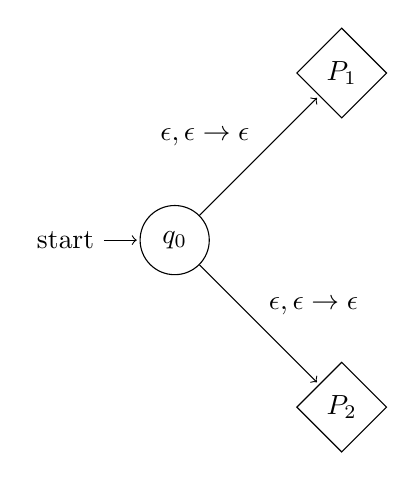
\begin{tikzpicture}[shorten >=1pt,node distance=3cm,on grid,auto]
  \node[state,initial] (q_0) {$q_0$};
  \node[state,diamond] (P_1) [above right=of q_0]{$P_1$};
  \node[state,diamond] (P_2) [below right=of q_0]{$P_2$};
  \draw[->]
  (q_0) edge node {$\epsilon,\epsilon\to\epsilon$} (P_1);
  \draw[->]
  (q_0)
  edge node {$\epsilon,\epsilon\to\epsilon$} (P_2);
  \end{tikzpicture}
      \end{figure}
    \end{proof}
  \item Let $L_1,L_2$ be \acp{CFL}. Then the concatenation \[
      \{w_1w_2 \mid w_1\in L_1, w_2 \in L_2\}
    \]
    is a \ac{CFL}.
    \begin{proof}
      The languages $L_1$ and $L_2$ are \aclp{CFL}, so there exist \acp{CFG}
      $G_1,G_2$ with start symbols $S_1,S_2$ that produce them. Suppose, without loss of generality, that
      $G_1,G_2$ have no nonterminal symbols in common (if they do, then we can rename
      them). Consider the grammar $S \rightarrow S_1S_2$. Then, this is a
      context free grammar, and its language is the concatenation of $L_1$ and
      $L_2$. So, the concatenation of $L_1$ and $L_2$ is a \ac{CFL}.
    \end{proof}
  \item Let $L$ be a \ac{CFL}. Then,
    \[
      L^* = \bigcup_{i \geq 0}\{w_1 \dots w_k\dots w_i \mid w_k\in L\}
    \]
    is a \ac{CFL}.
    \begin{proof}
      The language $L$ is a \ac{CFL}, so there exists a \ac{CFG} $G$ with start
      symbol $S_1$ that produces it. Consider the grammar given by $S\rightarrow
      S_1S\mid\epsilon$. This is a \ac{CFG} that produces $L^*$, so it follows
      that $L^*$ is a \ac{CFL}.
    \end{proof}
    \item Intersection with regular languages~\cite{hopcroft07:_introd_autom_theor_languag_comput}.\todo{}
  \end{itemize}
\end{thm}

\begin{prob}[Emptiness]
  \label{prob:cfg:emptiness}
  Let $G$ be a context-free grammar. Is $L(G)=\varnothing$?
  \begin{proof}[Proof of Decidability]
    \todo{}
  \end{proof}
\end{prob}

\begin{prob}[Finite]
  Let $G$ be a context-free grammar. Is $L(G)$ finite?
  \begin{proof}[Proof of Decidability]
    \todo{}
  \end{proof}
\end{prob}

\begin{prob}[Regular Containment]
Take some context-free grammar $G$ and some regular language $R$. Is
$L(G)\subseteq R$?
\begin{proof}[Proof of Decidability]
  We have that $L(G)\subseteq R$ if and only if
  $\overline{L(G)}\cup R = \Sigma^*$. So, it follows that $L(G)$ is contained by
  $R$ if and only iff $\overline{\overline{L(G)}\cup R} = \varnothing$. By
  DeMorgan's laws, we have that this is equivalent to the statement
  $L(G)\cap \overline{R} = \varnothing$. Regular languages are closed under
  complement and context-free languages are closed under intersection with a
  regular language, so it follows that $L(G)\cap \overline{R}$ is a context free
  language. So the problem of containment by a regular language is reducible to
  Problem~\ref{prob:cfg:emptiness}, the problem of emptiness, which is
  decidable. So, the problem of containment by a regular language is decidable.
\end{proof}

\end{prob}

\subsection{Undecidable Problems}
\begin{prob}[The Post Correspondence Problem]
  Consider some alphabet $\Sigma$ and two finite lists of words over $\Sigma$
  denoted $A = a_1,\dots,a_n$ and $B = b_1, \dots, b_n$. Then, does there exist
some sequence of indices $(i_k),$ for $1 \leq k \leq K$ and for
  $K\geq 1$, and with $1 \leq i_k \leq n$ for all $k$ such that
  \[
    a_{i_1}\dots a_{i_K} = b_{i_1}\dots b_{i_K}?
  \]
  \begin{proof}[Solution]
    This problem is shown to be undecidable through a reduction to the halting
    problem. The proof is technical, and involves encoding the computation
    history of a Turing machine on an input in such a way that the encoding satisfies the
    PCP if and only if the Turing machine accepts the input. It is described in
    detail by Sipser in his book \emph{Introduction to the Theory of Computation}
    \cite{sipser13:_introd_theor_comput}.
  \end{proof}
\end{prob}

The Post correspondence problem is a useful tool, because it allows us to
demonstrate the undecidability of problems without doing the complex reasoning
about Turing machines that the halting problem requires. We will now show the
undecidability of a variety of problems about context-free grammars through
reduction to the Post correspondence problem.

\begin{prob}[Disjointness]
  Let $P,Q$ be context-free grammars. Is $L(P)\cap L(Q) = \varnothing$?
  \begin{proof}[Proof of Undecidability]
    Consider the Post correspondence problem for two lists of words $A,B$. We
    construct two context free grammars from these lists as follows:
    \begin{equation*}
      \begin{split}
        G_A \rightarrow  &\;a_11 \\
        &\!\!\!\!\vdots \\
        G_A \rightarrow  &\;a_nn \\
        G_A \rightarrow  &\;a_1G_A1 \\
        &\!\!\!\!\vdots \\
        G_A \rightarrow  &\;a_nG_An \\
      \end{split}
      \qquad
      \begin{split}
        G_B \rightarrow  &\;a_11 \\
        &\!\!\!\!\vdots \\
        G_B \rightarrow  &\;a_nn \\
        G_B \rightarrow  &\;a_1G_B1 \\
        &\!\!\!\!\vdots \\
        G_B \rightarrow  &\;a_nG_Bn \\
      \end{split}
    \end{equation*}
    Then, we can observe that for some string $s$ to exist in both $L(G_A)$ and $L(G_B)$,
    it must be a solution to the Post correspondence for $A,B$. So, if $L(G_A)\cap
    L(G_B)=\varnothing$, then there are no solutions to the Post correspondence
    for $A,B$. So, it follows that the Post correspondence problem is reducible
    to the problem of the disjointness of context-free grammars, so since the
    Post correspondence problem is undecidable, it follows that the disjointness
    problem is undecidable.
  \end{proof}
\end{prob}

\begin{prob}[Universality]
  \label{prob:cfg:universality}
  Let $G$ be some context-free grammar over an alphabet $\Sigma$. Then, is
  \[
    L(G) = \Sigma^*?
  \]
  \begin{proof}[Proof of Undecidability]\todo{}
    
  \end{proof}
\end{prob}

\begin{defn}
We say that a \acl{CFG} is \emph{ambiguous} if there is more than one way to
apply the production rules to reach an accepted word, assuming a production rule
is always applied to the leftmost nonterminal symbol. This is equivalent to
stating that there is more than one parse tree that parses an accepted word.
\end{defn}

\begin{prob}[Ambiguity]
  Let $G$ be a context-free grammar. Is $G$ ambiguous?
  \begin{proof}[Proof of Undecidability]
    Consider the Post correspondence problem for two lists of words
    $A,B$. Construct their corresponding grammars $G_A,G_B$. Now, consider the
    grammar
    \[
      G \rightarrow G_A \vert G_B.
    \]
    It follows that the ambiguity of $G$ implies that a solution to the Post
    correspondence problem for $A,B$ exists, so the Post correspondence problem
    reduces to the ambiguity problem, so the ambiguity problem is undecidable.
  \end{proof}
\end{prob}
\cite{greibach66:_unsol_recog_linear_contex_free_languag}
\cite{Hopcroft1969}
\begin{prob}
  Let $G$ be a context free grammars. Is $L(G)$ regular?
  \begin{proof}[Proof of Undecidability]
    Note that $\Sigma^*$ is regular, so if $L(G)$ is not regular then it follows
    that $L(G)\neq \Sigma^*$. Additionally, universality is decidable within
    regular languages, because they are closed under complement and emptiness is
    decidable even within context-free grammars. So, we have that
    Problem~\ref{prob:cfg:universality} reduces to the regularity problem. It
    follows that the regularity problem is undecidable.
  \end{proof}
\end{prob}
\begin{prob}[Equality]
  Let $G_1,G_2$ be context free grammars. Is $L(G_1)=L(G_2)$?
  \begin{proof}[Proof of Undecidability]
    Note that $\Sigma^*$ is regular, so it is also a context-free. So,
    we have that Problem~\ref{prob:cfg:universality} reduces to the equality
    problem. It follows that the equality problem is undecidable.
  \end{proof}
\end{prob}
\begin{prob}[Inclusion]
  Let $G_1,G_2$ be context free grammars. Is $L(G_1)\subseteq L(G_2)$?
  \begin{proof}[Proof of Undecidability]
    As before, note that $\Sigma^*$ is regular, so it is also a
    context-free. Additionally, observe that for any grammar $G$, $L(G)\subseteq
    \Sigma^*$. So,
    we have that Problem~\ref{prob:cfg:universality} reduces to the inclusion
    problem, since $\Sigma^* \subseteq L(G) \implies \Sigma^* = L(G)$. It follows that the inclusion problem is undecidable.
  \end{proof}
\end{prob}

\subsubsection{Problems decidable for DCFLs}
\cite{ginsburg65:_deter}
\begin{defn}
  A \ac{DCFL} is a language accepted by a
  \acl{DPDA}.
\end{defn}

\begin{thm}[Closure Properties]
  \label{dcfl:complement}
  If $L$ is \ac{DCFL}, then $\overline{L}$ is a
  \ac{DCFL}.
  \begin{proof}
    Let $L$ be a \ac{DCFL}. Then, there exists some \ac{DPDA} $P$ that
    recognizes $L$. We can construct a new \ac{DPDA} $P'$ by complementing the
    accepting states of $P$. Because $P$ is a \ac{DPDA} and thus is only in one
    state at a time, $P'$ will recognize $\overline{L}$ and thus $\overline{L}$
    is a \ac{DCFL}. This would not hold if $P$ were only a \ac{PDA}, since a
    nondeterministic \ac{PDA} accepts if \emph{any} branch ends on an accepting
    state, and thus complementing the accepting states would not recognize the
    complement of the originally recognized language.
\end{proof}
\end{thm}

\begin{prob}
  Let $L$ be a \ac{DCFL}. Is $L = \Sigma^*$?
  \begin{proof}[Proof of Decidability]
    We have that $L$ is a \ac{DCFL}, so by Theorem~\ref{dcfl:complement},
    $\overline{L}$ is also a $\ac{DCFL}$. By Problem~\ref{prob:cfg:emptiness},
    we have that whether $\overline{L}$ is empty is decidable, so it follows
    that the question of whether $L = \Sigma^*$ is also decidable.
  \end{proof}
\end{prob}

The decidability of the following problem was an open problem in the field of
computability theory from 1965, when it was introduced by Ginsburg and Greibach \cite{ginsburg65:_deter}. In 1997, when it was solved by G\'eraud S\'enizergues
\cite{senizergues_det_pd_decid}. A sketch of the proof follows. 

\begin{prob}[The Equivalence Problem for Deterministic CFGs]
  Let $L_1,L_2$ be deterministic context-free languages. Is $L_1=L_2$?
\todo{}
\end{prob}

\section{Turing Degrees}
In Subsection~\ref{subsec:reducibility}, we introduced the concept of
Turing reducibility, denoted by the symbol $\leq_T$. This symbol suggests some type of
ordering over the set of decision problems. In this section, we introduce that
partial ordering on the set of decision problems and examine its properties.

\begin{defn}
  Let $A$ and $B$ be decision problems. We say that $A$ and $B$ are
  \emph{mutually reducibile} and write $=_T$ if $A \leq_T B$ and $B \leq_T A$.
\end{defn}

\begin{fact}
  The relation $=_T$ is an equivalence relation.
\end{fact}

We call the equivalence classes produced by this relation \emph{Turing degrees}
or \emph{degrees of unsolvability}, a concept first introduced in
1944 by Emil Post~\cite{post44:_recur}. We write the set of all such degrees as $\mathcal{D}$.

\begin{fact}
  The relation $\leq_T$ is a partial ordering of $\mathcal{D}$.
\end{fact}

\begin{defn}
  An oracle machine for a degree $A$, denoted $\mathcal{O}_A$, is a Turing
  machine equipped with a function that is able to decide $A$.
\end{defn}

\begin{defn}
  A problem $P$ is called \emph{computably enumerable} or \emph{semidecidable}
  for some degree $d\in\mathcal{D}$ if there exists a problem $A\in d$ such that
  it is possible to construct an oracle machine $\mathcal{O}_A$ such that
  $\mathcal{O}_A$ halts for all the inputs where $P$ is true, and does not halt
  on all the inputs for which $P$ is false. If $A=\varnothing$, and so the
  oracle machine does not have an oracle, then we simply say that $P$ is
  computably enumerable, semidecidable, or \emph{Turing recognizable}.
\end{defn}
\begin{rem}
  The Halting problem, Problem~\ref{prob:halting}, is Turing recognizable. The
  machine that recognizes the problem simply simulates the input machine.
\end{rem}

While it is simple to explicitly state problems lying in the lower degrees,
in order to more easily study the general structure of $\mathcal{D}$, we
introduce a new operator, \emph{jump}, that increments Turing degrees. Much of
the behavior of this operator was shown in a join paper by Kleene and Post~\cite{kleene54_upper_semi_lattic_degrees_recur_unsol}.

\begin{defn}
  The jump of $A$, denoted $A'$, is degree of the halting problem for oracle
  machines for $A$.
\end{defn}

The jump operator has many properties that make it convenient for studying the
Turing degrees, which are listed below. Further commentary on the jump operator
and its properties is available in Robert Soare's book \emph{History of Computability}~\cite{soare16_turin_comput}.
\begin{fact}
  The jump operator has many properties that make it convenient for studying the
Turing degrees, some of which are listed below. Further commentary on the jump operator
and its properties is available in Robert Soare's book \emph{History of Computability}~\cite{soare16_turin_comput}.
  \begin{itemize}
  \item $A'$ is computably enumerable in $A$.
  \item $A' \not\leq_T A$.
  \item If $B=_TA$ then $B'=_TA'$.
  \end{itemize}
\end{fact}

One of the earliest questions about the structure of the Turing degrees was
Post's Problem, first posed in 1944~\cite{post44:_recur}. It was solved
independently by Friedberg and Mucnik in the late 1950s using a technique
called the ``priority method''~\cite{Friedberg236, muchnik1956unsolvability}. A solution that does not
involve a priority argument was provided by Ku\v{c}era in 1986~\cite{Kucera:1986:APS:22416.22462}.

\begin{prob}[Post's Problem]  
  Does there exist a computably enumerable degree strictly between $0$ and $0'$?
  % Marchenkov 1976
  % Independently by Friedberg 57, Mucnik 56/58 using priority method
  % Priority free solution Kucer 1986''
  % ``Natural'' solns don't exist
\end{prob}

\subsection{Properties and Structure}


\begin{lem}
  \label{lem:deg_count}
  Every Turing degree is of cardinality $\aleph_0$.
  \begin{proof}
    We have that since every Turing machine can be expressed as a finite string over
    $\{0,1\}$, it can be expressed as a finite subset of $\mathbb{N}$. So, it follows
    that for any given oracle, there are at most $\aleph_0$ oracle machines, so
    at most $\aleph_0$ problems are decidable for any Turing degree.
    \par
    Now that an upper bound has been established,  we show that the cardinality
    of each degree is exactly $\aleph_0$.\todo{}
  \end{proof}
\end{lem}


\begin{lem}
  The set $\mathcal{D}$ is of cardinality $2^{\aleph_0}$.
  \begin{proof}
    First, observe that the cardinality of $\mathcal{D}$ is at most
    $2^{\aleph_0}$, since it is a set of sets of decision problems and there are
    at most $2^{\aleph_0}$ decision problems since decision problems are subsets
    of $\mathbb{N}$.\par Now, recall from Lemma~\ref{lem:deg_count} that each
    degree contains $\aleph_0$ decision problems. From this, it follows that
    there must be at least $2^{\aleph_0}$ degrees. So, we have that $\lvert \mathcal{D} \rvert=2^{\aleph_0}$.
  \end{proof}
\end{lem}

% Myhill 56 c.e.lattice
\begin{defn}
  A partially ordered set $S$ is said to form an \emph{upper semilattice} if, for every
 $x,y\in S$, there exists some element $z\in S$ such that $z \geq x,y$ and
 for all $w\in A$ such that $w\geq x,y$, we have that $w \geq z$. In other
 words, $x$ and $y$ have a supremum.
\end{defn}

\begin{defn}
  A partially ordered set $S$ is said to form a \emph{lattice} if all pairs
  $\{x,y\}\in S$ have both an infinum and a supremum.
\end{defn}


\begin{thm}
  \label{thm:up_sem}
  $\mathcal{D}$ forms an upper semilattice.
  % Kleene-Post 54 Degrees upper semi-lattice, jump an operator on degrees
    \begin{proof}
    Observe that it is sufficient to prove that every two degrees have a
    supremum. Let $A,B\in \mathcal{D}$ and  $P_1\in A, P_2 \in B$. Consider the operation
    \[
      A\vee B = \deg\left( \{2n \mid n \in P_1\}\cup\{2n+1\cup n\in P_2\} \right),
    \]
    where $\deg(A)$ is the Turing degree of $A$. Now, we show that $A\vee B = \sup(A,B)$.\par First, we show that
    $A,B \leq_T A \vee B$. This is equivalent to showing
    that problems in $A$ and $B$ are decidable by oracle machines for $A\vee
    B$. But simple construction gives oracle machines that can decide $P_1,P_2$
    given an oracle for $A\vee B$: for any $n$, if $2n\in A\vee B$ then
    $n\in P_1$, and if $2n+1\in A\vee B$ then $n\in P_2$. This holds for any
    $P_1,P_2$, so it follows that $A,B \leq_T A \vee
    B$. \par Now, let $W\in \mathcal{D}$ such that $W \geq
    A,B$ and let $P\in A\vee B$. Then, we have that for every $n$, we can
    determine whether $n\in P$ by determining whether $n$ is even and
    $\frac{n}{2}\in P_1$ or odd and $\frac{n-1}{2}\in P_2$. Since both the parity
    of a number and $P_1$ and $P_2$ are decidable in $W$, it follows that
    $A\vee B$ is decidable in $W$, and thus $A\vee B \leq_T W$. So, it follows
    that $A\vee B = \sup(A,B)$. This holds for all $A,B\in\mathcal{D}$, so it
    follows that $\mathcal{D}$ forms an upper semilattice.  
  \end{proof}
\end{thm}

\begin{fact}
  \label{fact:not_lat}
  $ \mathcal{D}$ does not form a lattice.
\end{fact}
\begin{rem}
Theorem~\ref{thm:up_sem} and Fact~\ref{fact:not_lat} were first shown in
Kleene's \emph{The Upper Semi-Lattice of Degrees of Recursive
  Unsolvability}~\cite{kleene54_upper_semi_lattic_degrees_recur_unsol}. A simpler proof
of Fact~\ref{fact:not_lat} is available in Robert Soare's book \emph{Turing Computability}~\cite[pp.~142--144]{soare16_turin_comput}.
\end{rem}

\begin{thm}
  Existence of minimal degrees
  % Spector 56,Shoenfield 66 (Better)
  \cite{spector56_degrees_recur_unsol}
  \cite{shoenfield66_theor_minim_degrees}
\end{thm}

\begin{thm}
  The c.e. degrees are dense
  \cite{sacks64:_recur_enumer_degrees_dense}
\end{thm}

Homogeneity problems
% Feiner 1970, Shore 1979

Theory of D Undecidable


Theory of D equivalent to to second-order arithmetic \cite{simpson77:_first_order_theor_degrees_recur_unsol}

% \subsection{Turing Degrees of Problems related to CFGs}
% \cite{REEDY197577}




\section*{Acknowledgments}
It is a pleasure to thank my mentor, Ronno Das, for supervising this project and
providing valuable feedback and advice. I would also like to thank Peter May for
organizing this REU, and Daniil Rudenko for running the Apprentice Program.

\printbibliography

\end{document}


%%% Local Variables:
%%% mode: latex
%%% TeX-master: t
%%% End:
